%!TEX root = ../../main.tex

\subsection{System Domænemodel}

\begin{figure}[H]
	\centering
	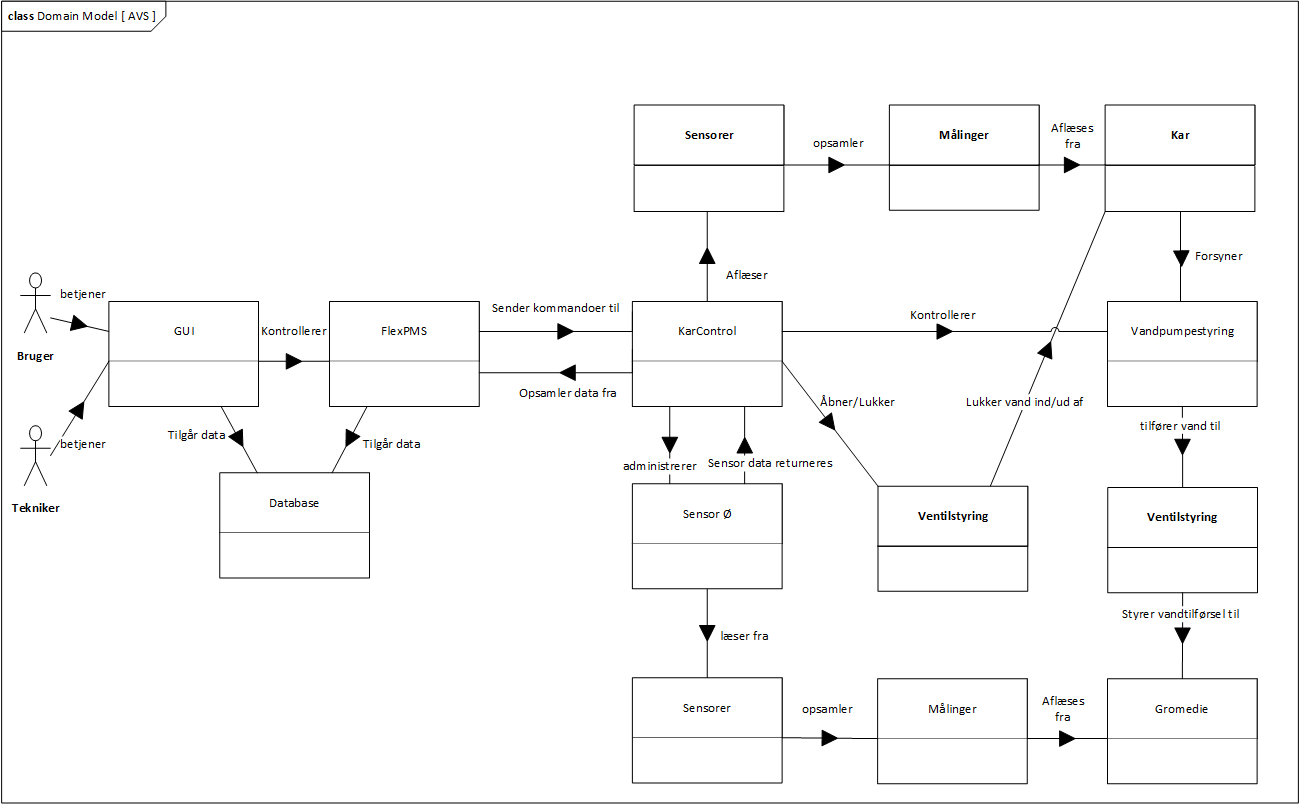
\includegraphics[width=0.82\textwidth]{Systemarkitektur/System/AVS_domain_model.png}
	\label{fig:System BDD}
	\caption{Domain model af AVS}
\end{figure}



\subsection{System BDD}

\begin{figure}[H]
	\centering
	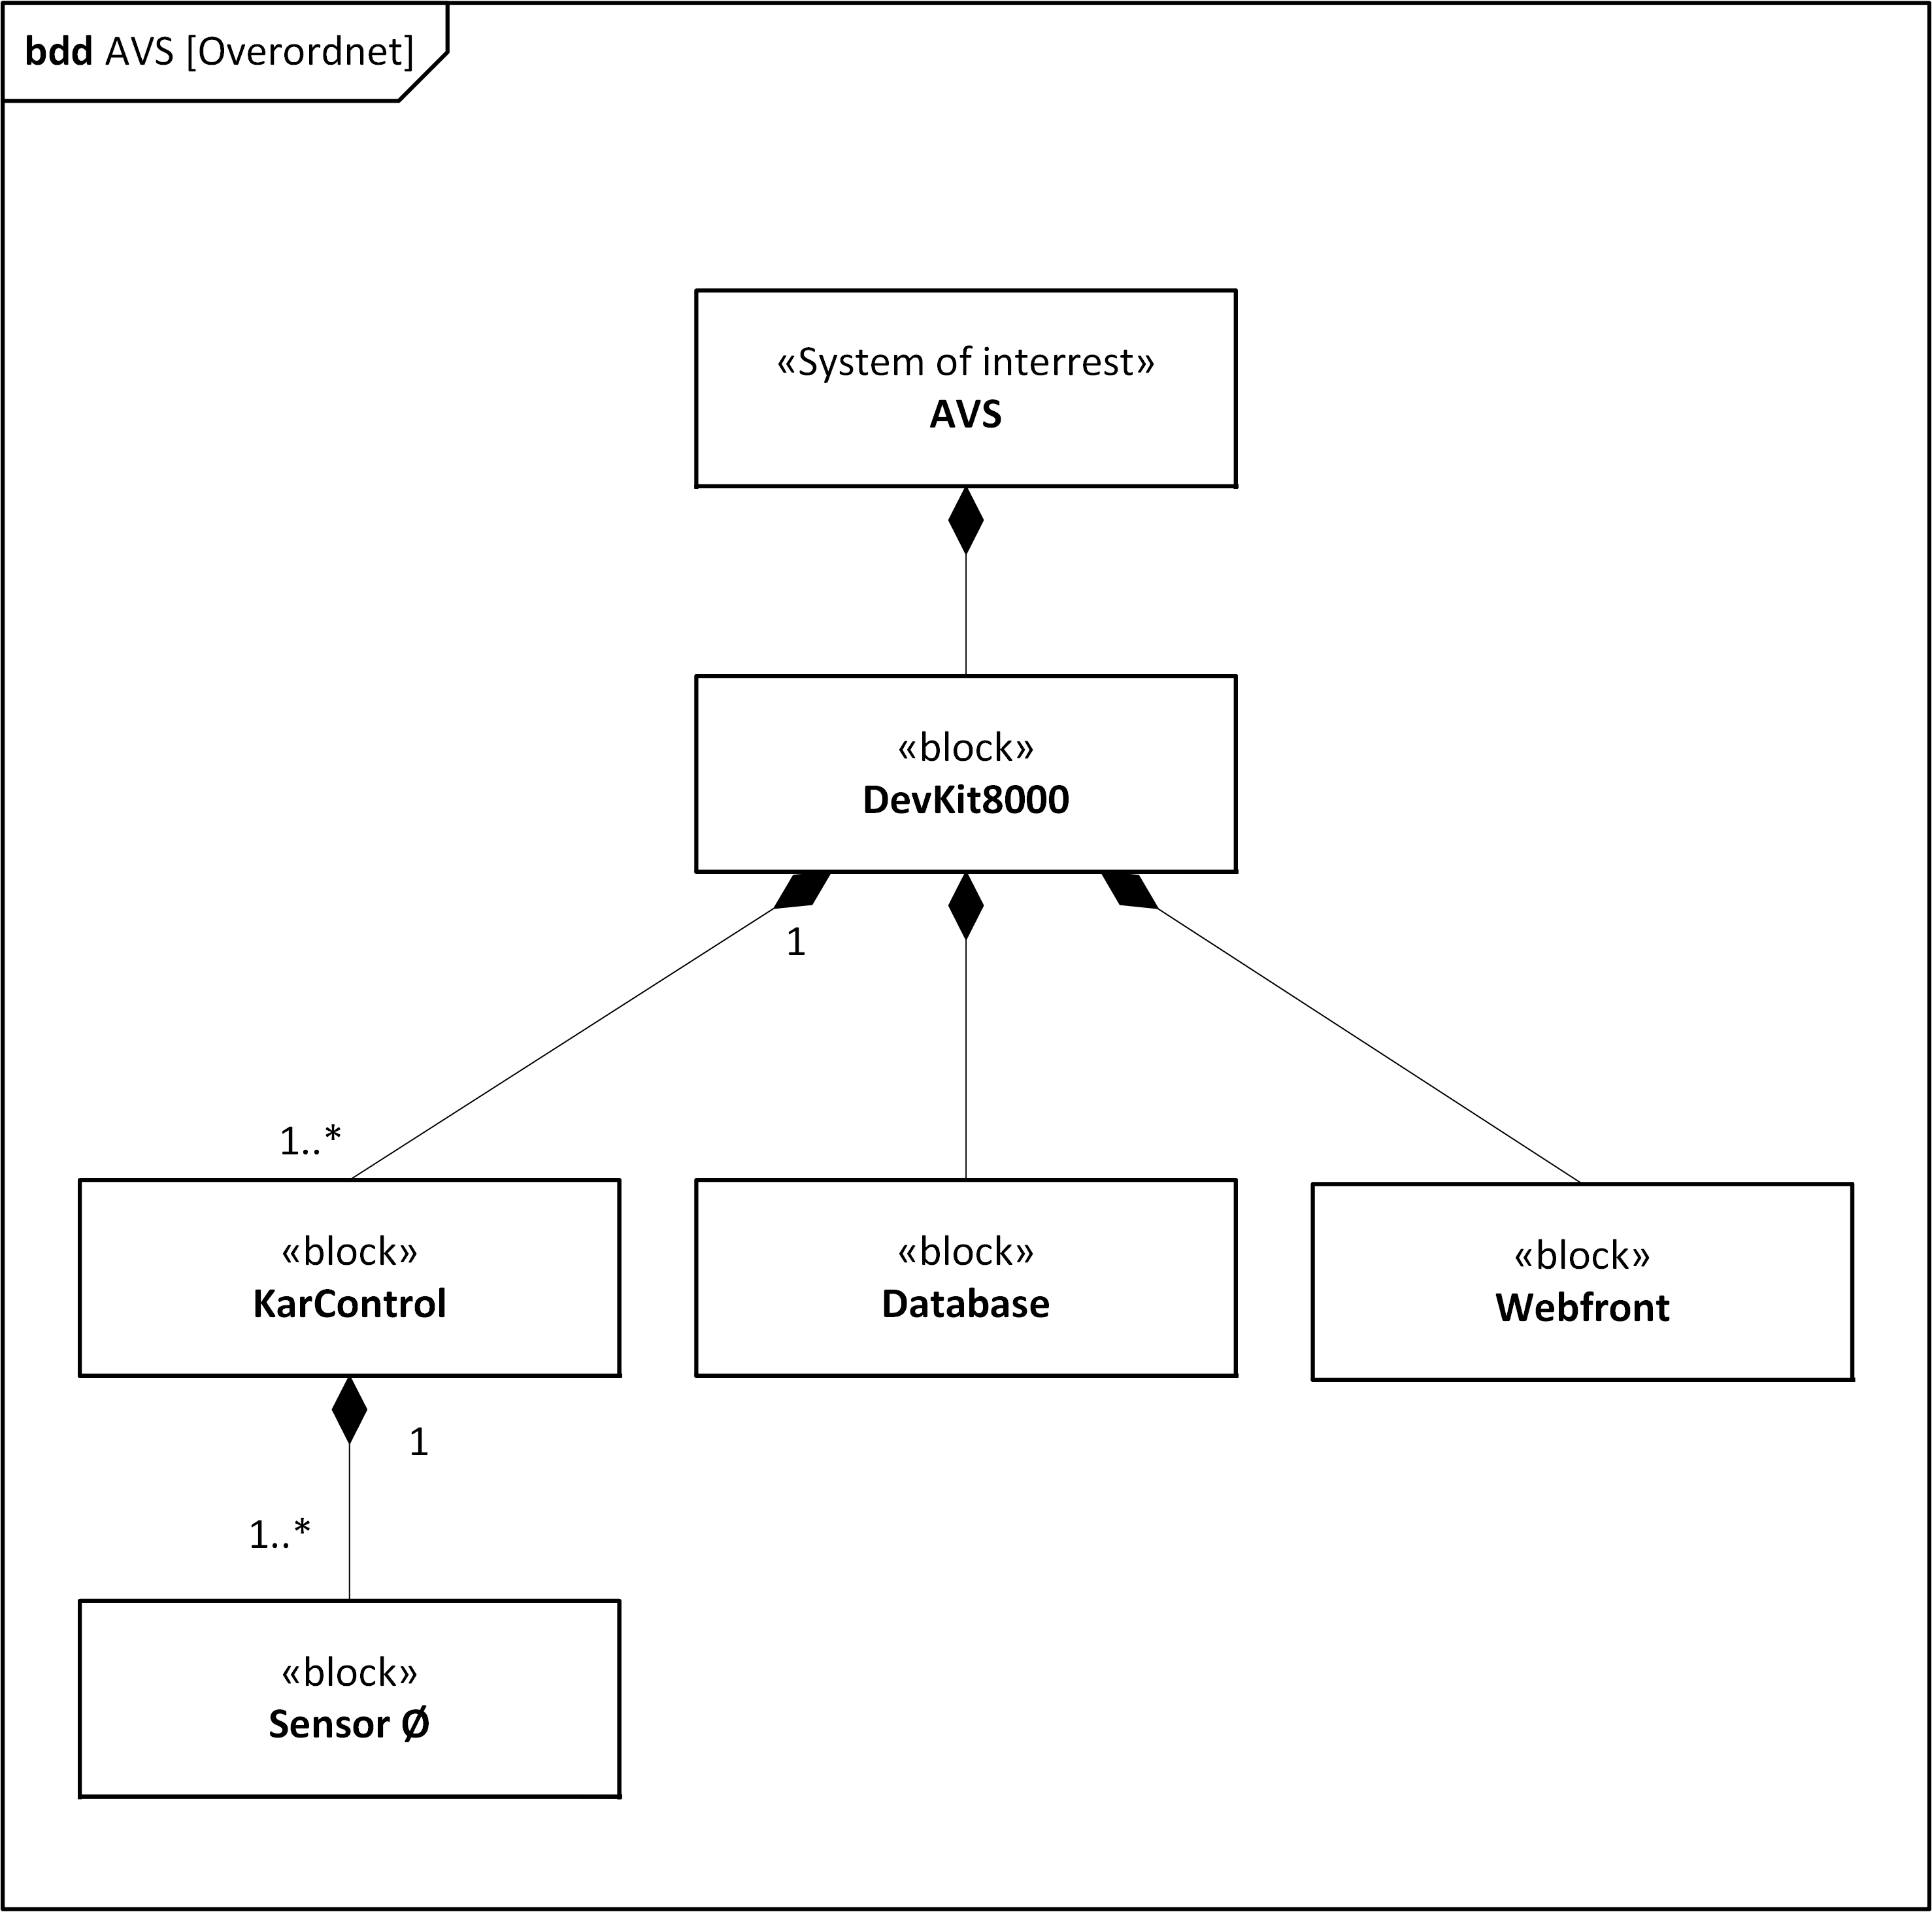
\includegraphics[width=0.82\textwidth]{Systemarkitektur/System/AVS_SystemdiagramBDD.png}
	\label{fig:System BDD}
	\caption{Block Definition Diagram af AVS}
\end{figure}

\subsubsection{CentralControl}
CentralControl er systemets centrale computer. Det er gennem dette delsystem, at brugerens interaktion bliver behandlet og formidlet videre til andre delsystemer. CentralControl driver en webserver med dertilhørende web-applikation (GUI), som tillader brugeren at interagere med systemet gennem sin web-browser. Webserveren kommunikerer med et stykke centralt software, FlexPMS.

\subsubsection{GUI}
GUI er den brugergrænseflade, som brugeren kan tilgå systemet gennem.

\subsubsection{FlexPMS}
FlexPMS (Flexible Plant Management System) softwaren er bindeleddet mellem GUI og de andre delsystemer. FlexPMS afvikles konstant på CentralControl, og håndterer at sende kommandoer til og opsamle data fra KarControl. FlexPMS kommunikerer med de andre delsystemer gennem enhedsdrivers, som er udviklet til – og installeret på – CentralControl.

\subsubsection{Database}
Databasen gemmer alle indstiller lavet af brugeren gennem GUI.

\subsubsection{KarControl}
KarControl er en styring, som formidler og håndterer al datakommunikation og kommandoer relateret til ét kar. KarControl formidler kommandoer sendt fra CentralControl videre til hardware koblet på det pågældende kar (f.eks. at åbne og lukke for ventiler), samt formidler måledata fra sensorer tilbage til CentralControl. KarControl ved hvilken pH-værdi karret skal have, samt hvilken koncentration af gødning og jordfugtighed planterne, der er tilkoblet karret, skal have. KarControl sørger selv for, at vedligeholde disse værdier. CentralControl giver KarControl besked, når der foretages ændringer af disse værdier.

\subsubsection{Sensor Ø}
Sensor Ø’er giver mulighed for at måle (f.eks. jordfugtighed) over et større areal ved, at Sensor Ø’erne spredes over området, hvor planterne gror, og har hver især tilsluttet sensorer. Dermed kan man måle jordfugtighed lokalt for området omkring Sensor Ø’en og styre vandtilførslen specifikt for planterne, som står i området.
\subsection{Allokeringsdiagram}

\begin{figure}[H]
	\centering
	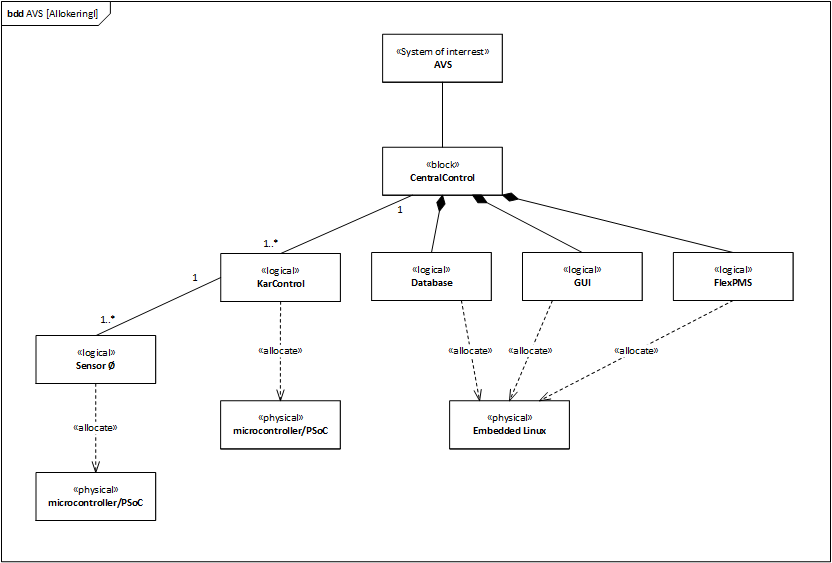
\includegraphics[width=0.82\textwidth]{Systemarkitektur/System/AVS_Allokeringsdiagram.png}
	\label{fig:System BDD}
	\caption{Allokeringsdiagram af AVS}
\end{figure}







